\section{Preliminary Results}

\begin{figure}[h]
\makebox[\textwidth][c]{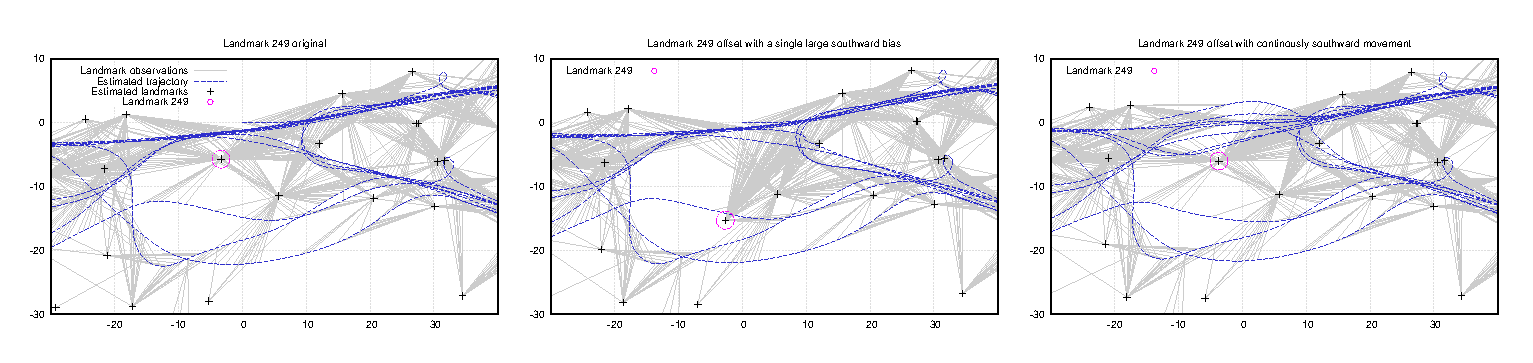
\includegraphics[width=1.1\textwidth]{fig/baseline-mm}}
\caption{Left: convergence chi-square is 17287. Middle: observations of
landmark 249 are displaced with a 10 meter southward bias; convergence
chi-square is 231898 indicating high uncertainty. Half of observations of 249
are rejected by max-mixture, while the trajectory suffers from slight
distortion with landmark 249 displaced by correct amount. Right: observation of 249 are
added with southward moving offsets with the total movement of 7 meter.
Convergence chi-square is 17807.}
\label{fig:baseline}
\end{figure}

In this section, we evaluate the max-mixture algorithm well-known for its
capability of handling a large amount of incorrect loop closures. Since the
max-mixture algorithm is a representative framework in the robust SLAM
literature, its performance against dynamic environments will have border
implication on later work. The evaluation is based on the Victoria Park dataset
with different crafted noises introduced on a single landmark (landmark 249).
The dataset contains 10607 measurements, 151 landmarks, and 6969 poses. Figure
\ref{fig:baseline} shows a local part of the trajectory and map estimation
obtained by the Max-Mixture algorithm on three instances of the dataset with
all observations of landmark 249 converted to unimodal max-mixture type. A
single large bias introduced in all observations of one landmark makes
Max-Mixture results slightly distorted but mostly recovered from the errors.
But the simulated errors of slowly moving landmark has largely distorted the
result of Max-Mixture.

This demonstrates how the max-mixture algorithm is unable to handle a locally
consistent moving landmark while capable of handling noise of large
displacement or spurious loop closures. An explanation for this is that each
clique of landmarks with coherent motion forms a plausible reference frame for
related observations. Inference based on each independent reference frame will
reach plausible estimate of robot trjectory and the map, however averaging over
a sum of different reference frames would lead to wrong conclusions.

